% % % % % % % % % % % % % % % % % % % % % % % % % % % % % % % % % % % % % % % % % % % %
%                                                                                     %
% Short Sectioned Assignment LaTeX Template Version 1.0 (5/5/12)                      %
% This template has been downloaded from: http://www.LaTeXTemplates.com               %
%                                                                                     %
% Original author:  Frits Wenneker (http://www.howtotex.com)                          %
%                                                                                     %
% Modified by: Fco Javier Sueza Rodríguez (fcosueza@disroot.org)                      %
%                                                                                     %
% Changes:                                                                            %
%	    - Custom Chapters, Sections and Subsections (titlesec package)                %
%           - Document type scrbook (oneside)                                         %
%           - Use babel-lang-spanish package and marvosym                             %
%           - Use hyperref, enumitem, tcolorbox and glossaries packages               %
%           - Use Time New Roman (mathptmx), Helvetic and Courier fonts               %
%                                                                                     %
% License: CC BY-NC-SA 3.0 (http://creativecommons.org/licenses/by-nc-sa/3.0/)        %
%                                                                                     %
% % % % % % % % % % % % % % % % % % % % % % % % % % % % % % % % % % % % % % % % % % % %

%-----------------------------------------------%
%	              Packages                  %
%-----------------------------------------------%

\documentclass[paper=a4, fontsize=11pt, oneside]{scrbook}

% ---- Text Input/Output ----- %

\usepackage[T1]{fontenc}
\usepackage[utf8]{inputenc}
\usepackage{mathptmx}
\usepackage[scaled=.92]{helvet}
\usepackage{courier}
\usepackage[indent=12pt]{parskip}

\usepackage{geometry}
\geometry{verbose,tmargin=3cm,bmargin=3cm,lmargin=2.6cm,rmargin=2.6cm}

% ---- Language ----- %

\usepackage[spanish]{babel}
\usepackage{marvosym}

% ---- Another packages ---- %

\usepackage{amsmath,amsfonts,amsthm}
\usepackage{graphics,graphicx}
\usepackage{titlesec}
\usepackage{fancyhdr}
\usepackage{tcolorbox}
\usepackage{hyperref}
\usepackage{enumitem}
\usepackage[automake]{glossaries}

%--------------------------------------------------------------------%
%                      Customizing Document                          %
%--------------------------------------------------------------------%


% ----------- Custom Chapters, Sections and Subsections -------------- %

\titleformat{\chapter}[display]
			{\bfseries\Huge}
			{Tema \ \thechapter} {0.5ex}
			{\vspace{1ex}\centering}

\titleformat{\section}[hang]
			{\bfseries\Large}
			{\thesection}{0.5em}{}

\titleformat{\subsection}[hang]
			{\bfseries\large}
			{\thesubsection}{0.5em}{}

\titleformat{\subsubsection}[hang]
			{\bfseries\large}
			{\thesubsubsection}{0.5em}{}

\hypersetup{
    colorlinks=true,
    linkcolor=black,
    urlcolor=magenta
}

% ------------------- Custom heaaders and footers ------------------- %

\pagestyle{fancyplain}

\fancyhead[]{}
\fancyfoot[L]{}
\fancyfoot[C]{}
\fancyfoot[R]{\thepage}

\renewcommand{\headrulewidth}{0pt} % Remove header underlines
\renewcommand{\footrulewidth}{0pt} % Remove footer underlines

\setlength{\headheight}{13.6pt} % Customize the height of the header

% --------- Numbering equations, figures and tables ----------------- %

\numberwithin{equation}{section} % Number equations within sections
\numberwithin{figure}{section} % Number figures within sections
\numberwithin{table}{section} % Number tables within sections

% ------------------------ New Commands ----------------------------- %

\newcommand{\horrule}[1]{\rule{\linewidth}{#1}} % Create horizontal rule command


%----------------------------------------------------------------------------------------
%	TÍTULO Y DATOS DEL ALUMNO
%----------------------------------------------------------------------------------------

\title{
\vspace{10ex}
\normalfont \normalsize
\Huge \textbf{Tarea 5: Administración Básica del Sistema (Windows II)}
}
\author{Francisco Javier Sueza Rodríguez}
\date{\normalsize\today}

%----------------------------------------------------------------------------------------
%                                     DOCUMENTO
%----------------------------------------------------------------------------------------
\begin{document}

\maketitle

\thispagestyle{empty}

\vspace{68ex}

\begin{center}
    \begin{tabular}{l l}
        \textbf{Centro}: & IES Aguadulce \\
        \textbf{Ciclo Formativo}: & Desarrollo Aplicaciones Web (Distancia)\\
        \textbf{Asignatura}: & Sistemas Informáticos\\
        \textbf{Tema}: & Tema 5 -  Administración Básica del Sistema (Windows II)\\
    \end{tabular}
\end{center}

\newpage

\tableofcontents

\newpage

\listoffigures

\newpage

\section{Caso Práctico}
María ya tiene instalado en los equipos de la empresa AguadulSoft el sistema operativo y ahora es el momento de empezar a administrar el sistema para configurarlo y ponerlo en marcha para su utilización. Como es la primera vez, Juan le va a ayudar en el proceso de administración básica del sistema. Ada será la que les dé el visto bueno.

\section{Actividades}

\subsection{Actividad 1: Estructura Departamental}
\subsubsection{Enunciado}

Crea la siguiente estructura departamental de carpetas colgando directamente de la raíz del disco en la que está instalado Windows 10. Crea primero la carpeta "AguadulSoft" y dentro de esta las demás:

    \begin{figure}[H]
    \centering
    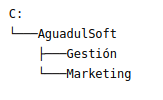
\includegraphics[scale=1]{estructura-enunciado.png}
    \caption{Estructura de carpetas a crear}
\end{figure}

Introduce dos archivos, un documento y una imagen, en la carpeta de cada departamento (Gestión y Marketing) y nómbralos como tipoArchivo\_nombreDepartamento (por ejemplo, en la carpeta ``Gestión'' el documento sería nombrado como ``documento\_gestión'' y la imagen como ``imagen\_gestión'').

\textbf{Capturas}:

\begin{itemize}
    \item Muestra de la estructura departamental de carpetas y de su ubicación.
    \item Archivos de cada carpeta.
\end{itemize}

\subsubsection{Solución}
\begin{enumerate}
    \item En primer lugar hemos creado los directorios desde la interfaz gráfica.

    \begin{figure}[H]
        \centering
        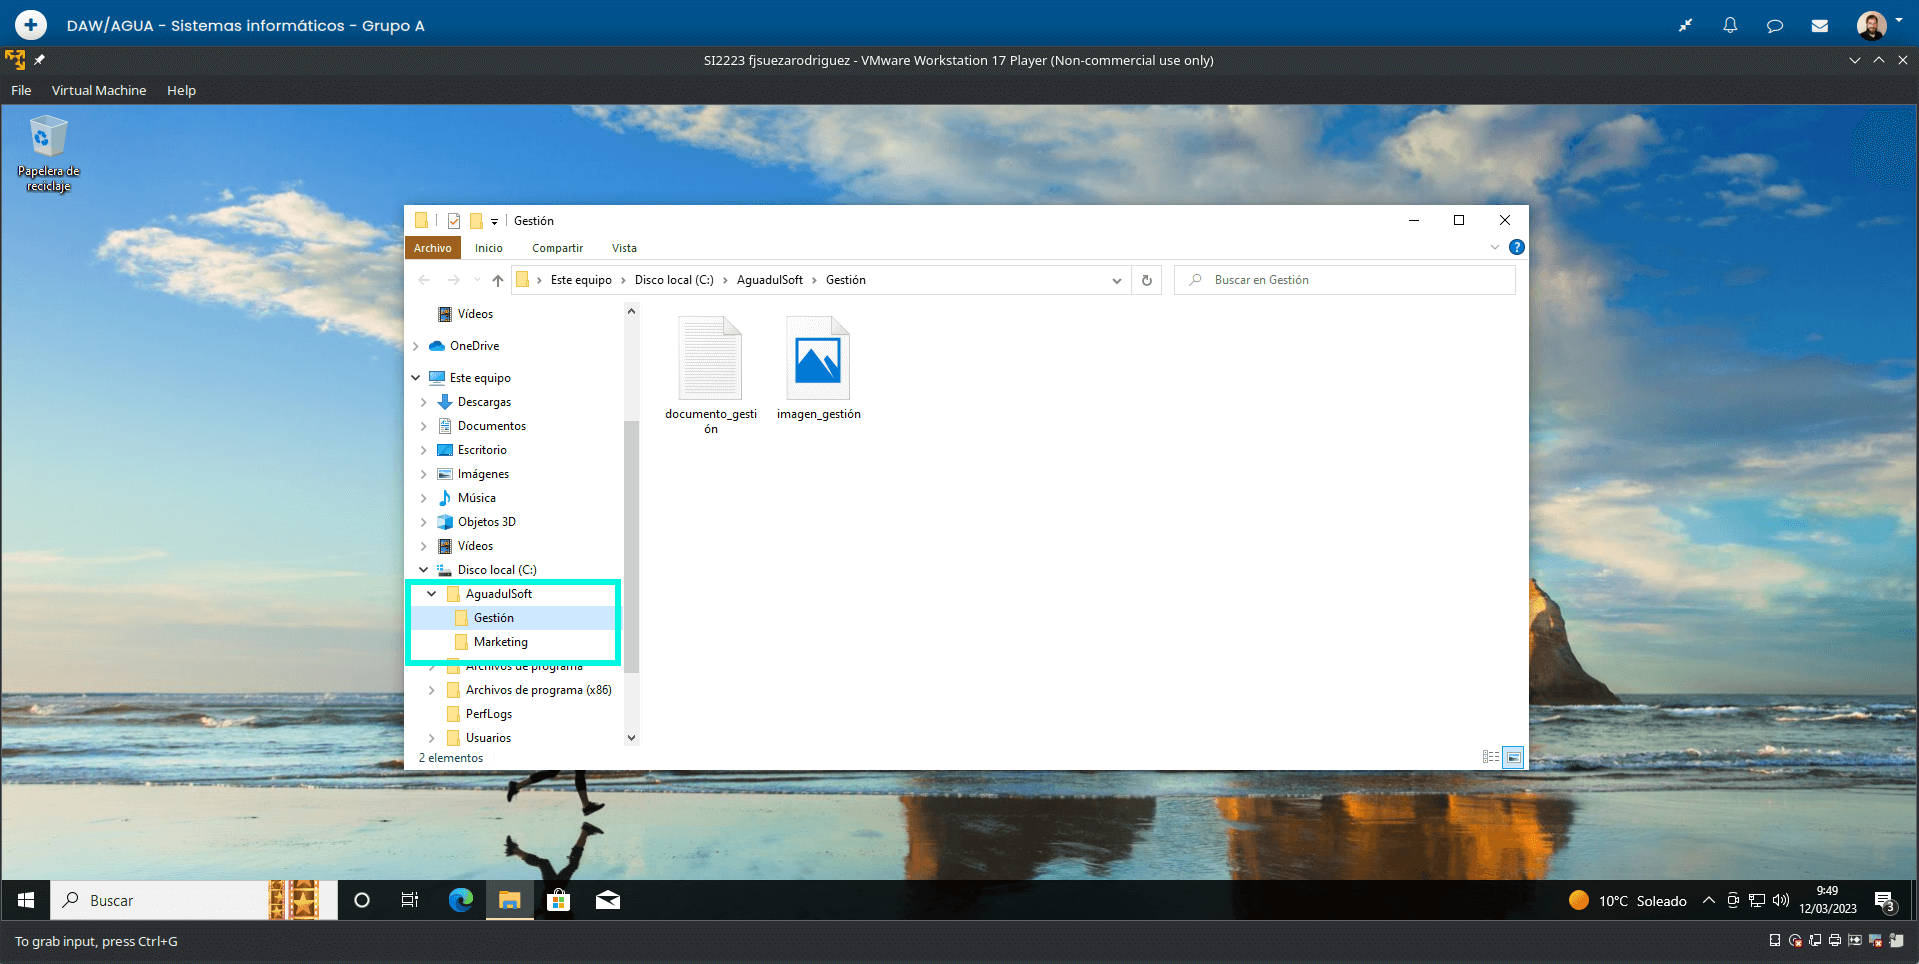
\includegraphics[scale=0.19]{estructura.png}
        \caption{Estructura de directorios creada}
    \end{figure}

    \item A continuación, hemos añadido 2 archivos a cada directorio creado, como se especifica en el enunciado. Se ha usado también la opción ``\textbf{Nuevo ---> archivo de texto/imagen de mapa de bits}'' para crear estos archivos.

    \begin{figure}[H]
        \centering
        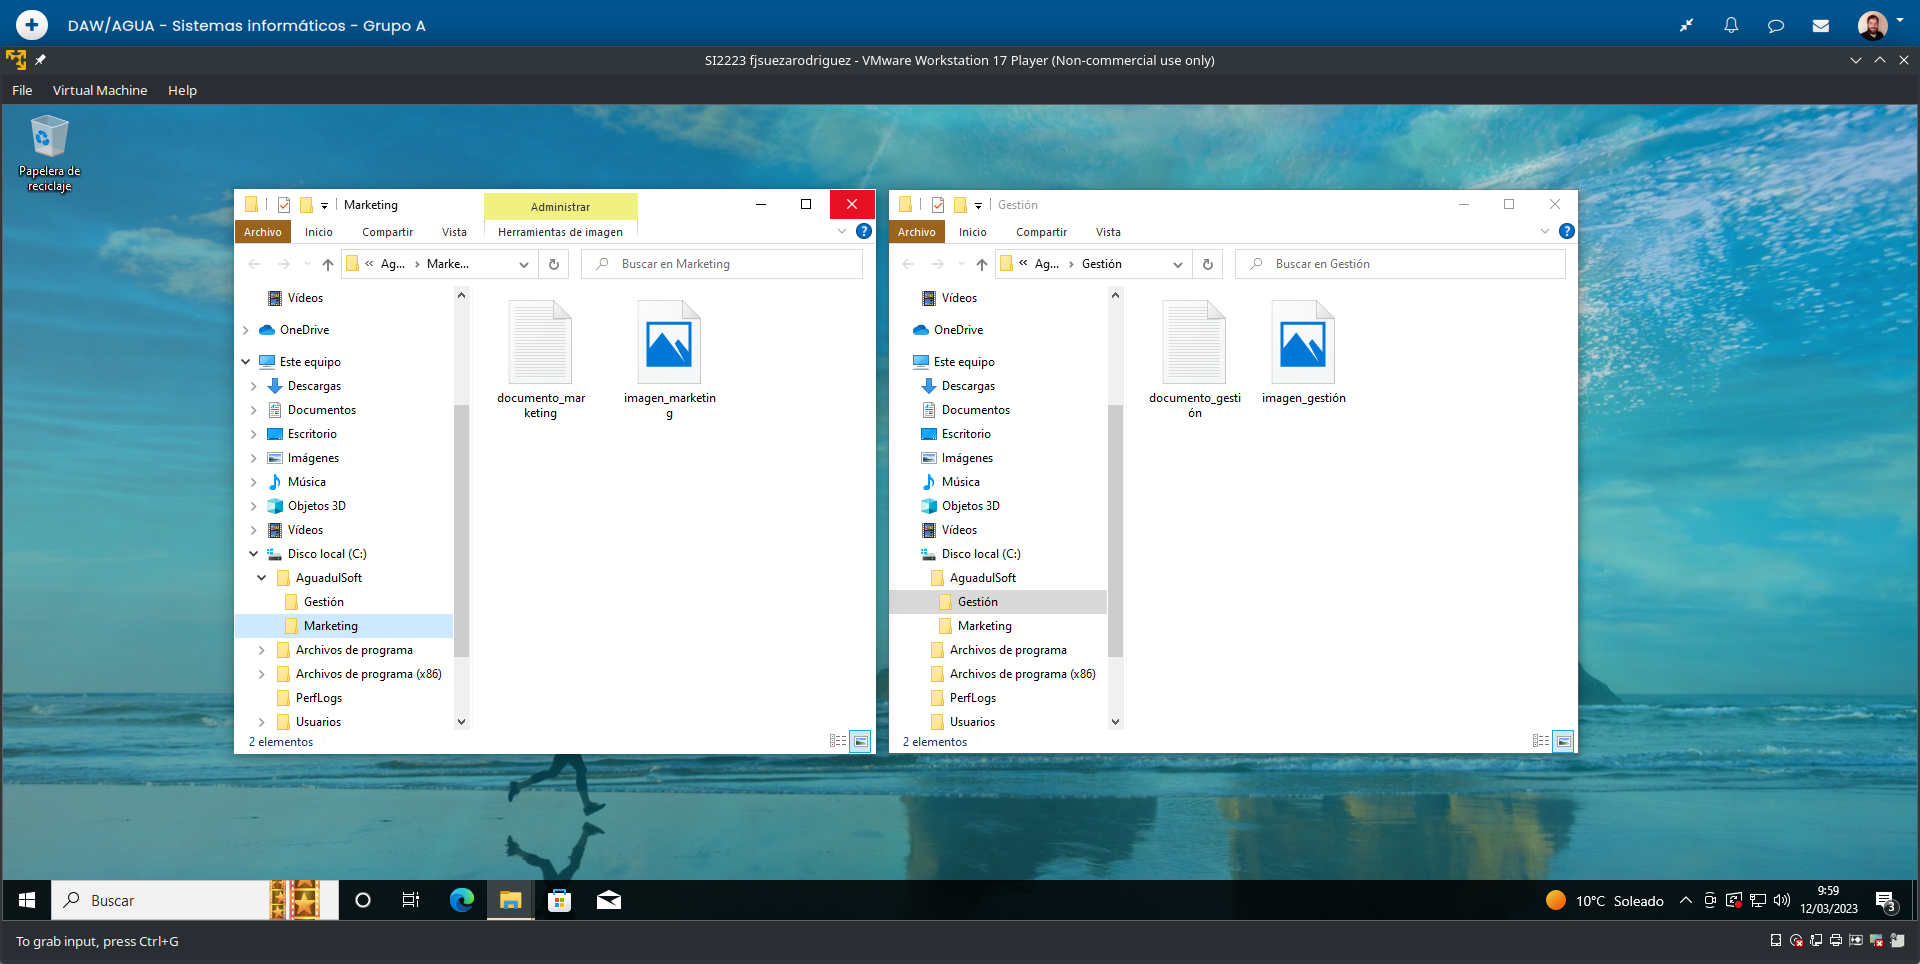
\includegraphics[scale=0.23]{estructura-archivos.png}
        \caption{Archivos creados es las carpetas Marketing y Gestión}
    \end{figure}
\end{enumerate}

\subsection{Actividad 2: Cuentas de Usuario Locales}

\subsection{Enunciado}

\begin{enumerate}[label=2.\alph*)]
    \item \textbf{Creación de Usuarios}: crea las siguientes cuentas de usuarios locales (con privilegios limitados):
    \begin{itemize}
        \item Gestión: Graciela Góngora y Genaro García.
        \item Marketing: Matías Martínez y Marta Mejías.
    \end{itemize}

    Nombra cada cuenta de usuario como InicialNombreApellido e introduce en el campo ``Nombre completo'' su nombre y apellido completos y en el campo ``Descripción'' el nombre del departamento al que pertenece (por ejemplo, el usuario ``Graciela Góngora'' del departamento ``Gestión'' sería nombrado como ``ggongora'' y en sus campos se introduciría ``Graciela Góngora'' en ``Nombre completo'' y ``Dpto. de Gestión'' en ``Descripción'').

    \textbf{Capturas}:
    \begin{itemize}
        \item Ventana/consola donde se crea un nuevo usuario (indica textualmente cómo se accede a dicha ventana).
        \item Introducción del nombre y campos "Nombre completo" y "Descripción" de la primera cuenta de usuario.
        \item Resumen de las cuentas de usuario creadas con sus respectivos nombres yitemize
    \end{itemize}

    \item \textbf{Creación de Grupos}: crea un grupo de usuarios para cada departamento, nómbralos con su nombre de departamento y en el campo ``Descripción'' introduce el texto ``Departamento de X'' donde X es el nombre del departamento (por ejemplo, el grupo de usuarios del departamento ``Gestión'' sería nombrado como ``Gestión'' y en su campo ``Descripción'' se introduciría ``Departamento de gestión'').

    Incluye en cada uno de ellos sus usuarios correspondientes, creados en la actividad anterior.

    \textbf{Capturas}:
    \begin{itemize}
        \item Ventana donde se crea un nuevo grupo de usuarios (indica textualmente cómo se accede a dicha ventana).
        \item Introducción del nombre y campo ``Descripción'' del primer grupo de usuarios.
        \item Asignación de los usuarios del primer grupo de usuarios.
        \item Resumen de los grupos de usuarios creados con sus respectivos nombres, campos y usuarios.
    \end{itemize}
\end{enumerate}

\subsubsection{Solución}

\begin{enumerate}
    \item En primer lugar, hemos \textbf{creado los usuarios solicitados} con los datos que se especifican en el enunciado. Hemos elegido la opción de crearlos mediante la aplicación \textbf{LUSRMGR.MSC}, ya que es la que proporciona la opciones de configuración más completas.

    Para acceder a esta aplicación, hemos ejecutado el comando \textbf{LUSRMGR.MSC} en consola, aunque se puede poner también en la barra de búsqueda de Windows y clickar en la aplicación que nos da como resultado. Una vez ahí, hemos pulsado en la opción ``\textbf{Acciones adicionales ---> Nuevo usuario}.

     \begin{figure}[H]
        \centering
        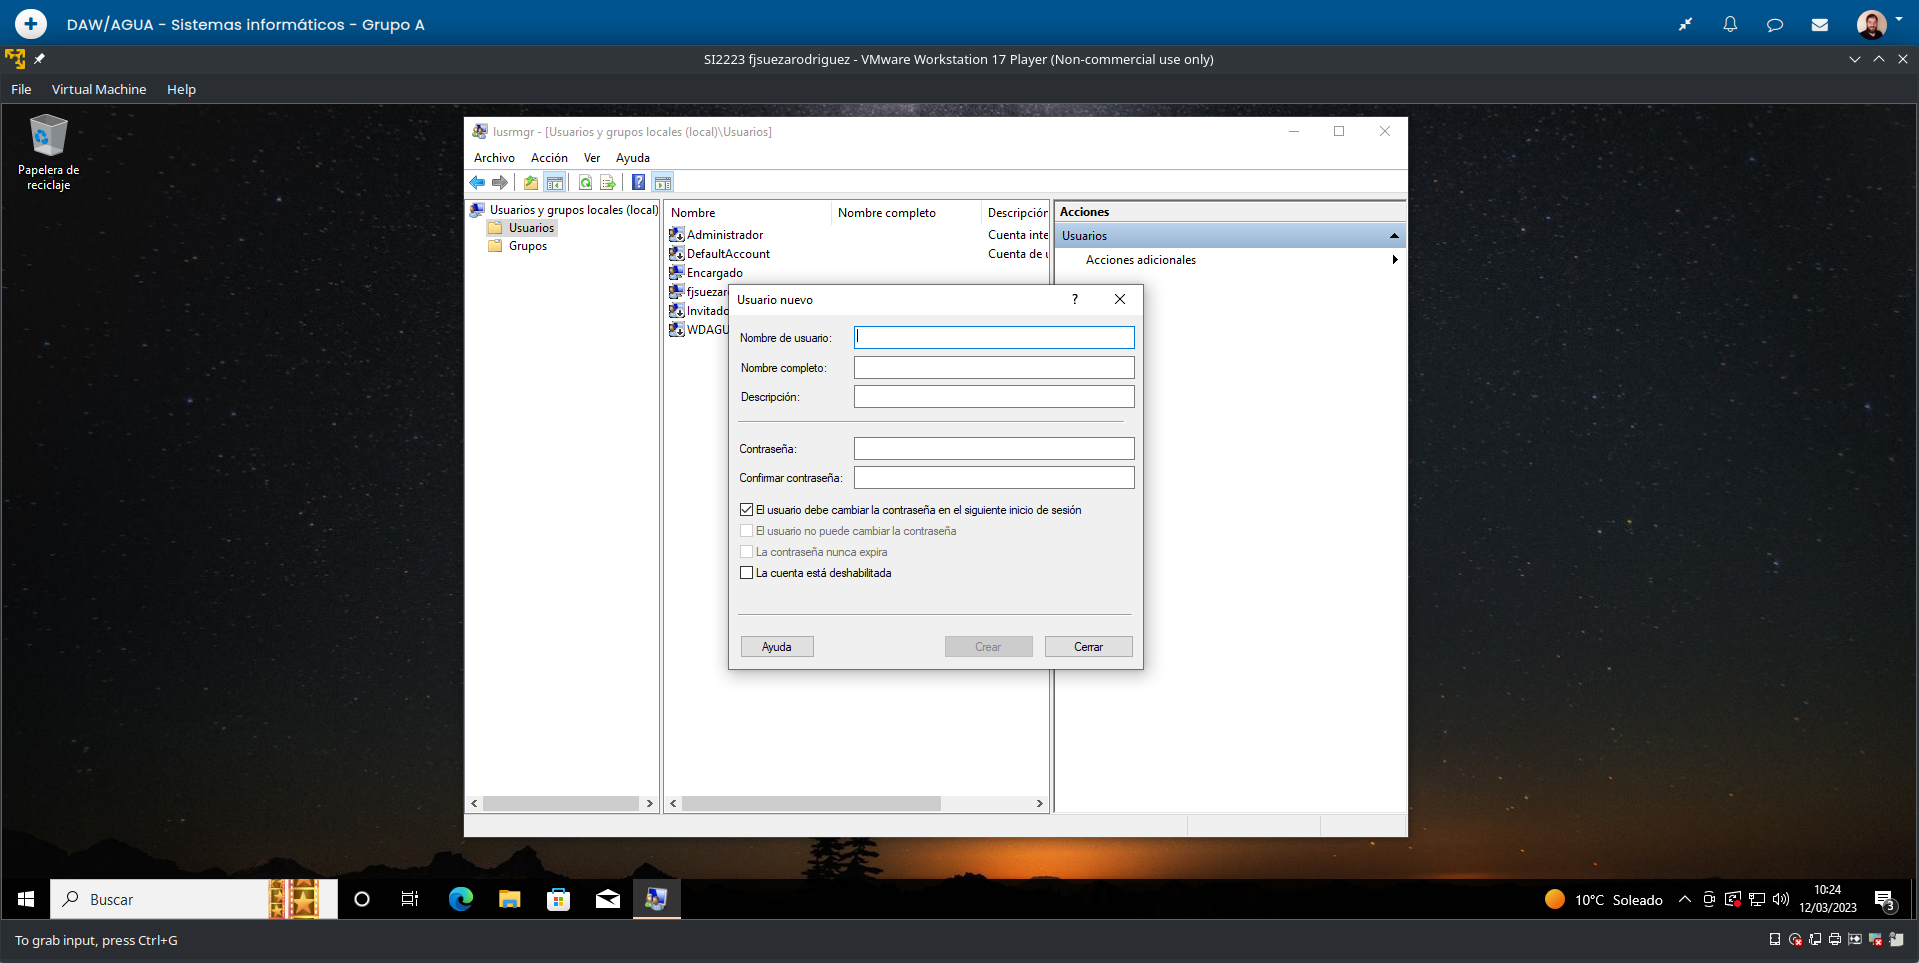
\includegraphics[scale=0.22]{usuarios-creacion.png}
        \caption{Ventana de creación de usuario}
    \end{figure}

    A continuación hemos introducido los datos solicitados, tal y como se explica en el enunciado.

    \begin{figure}[H]
        \centering
        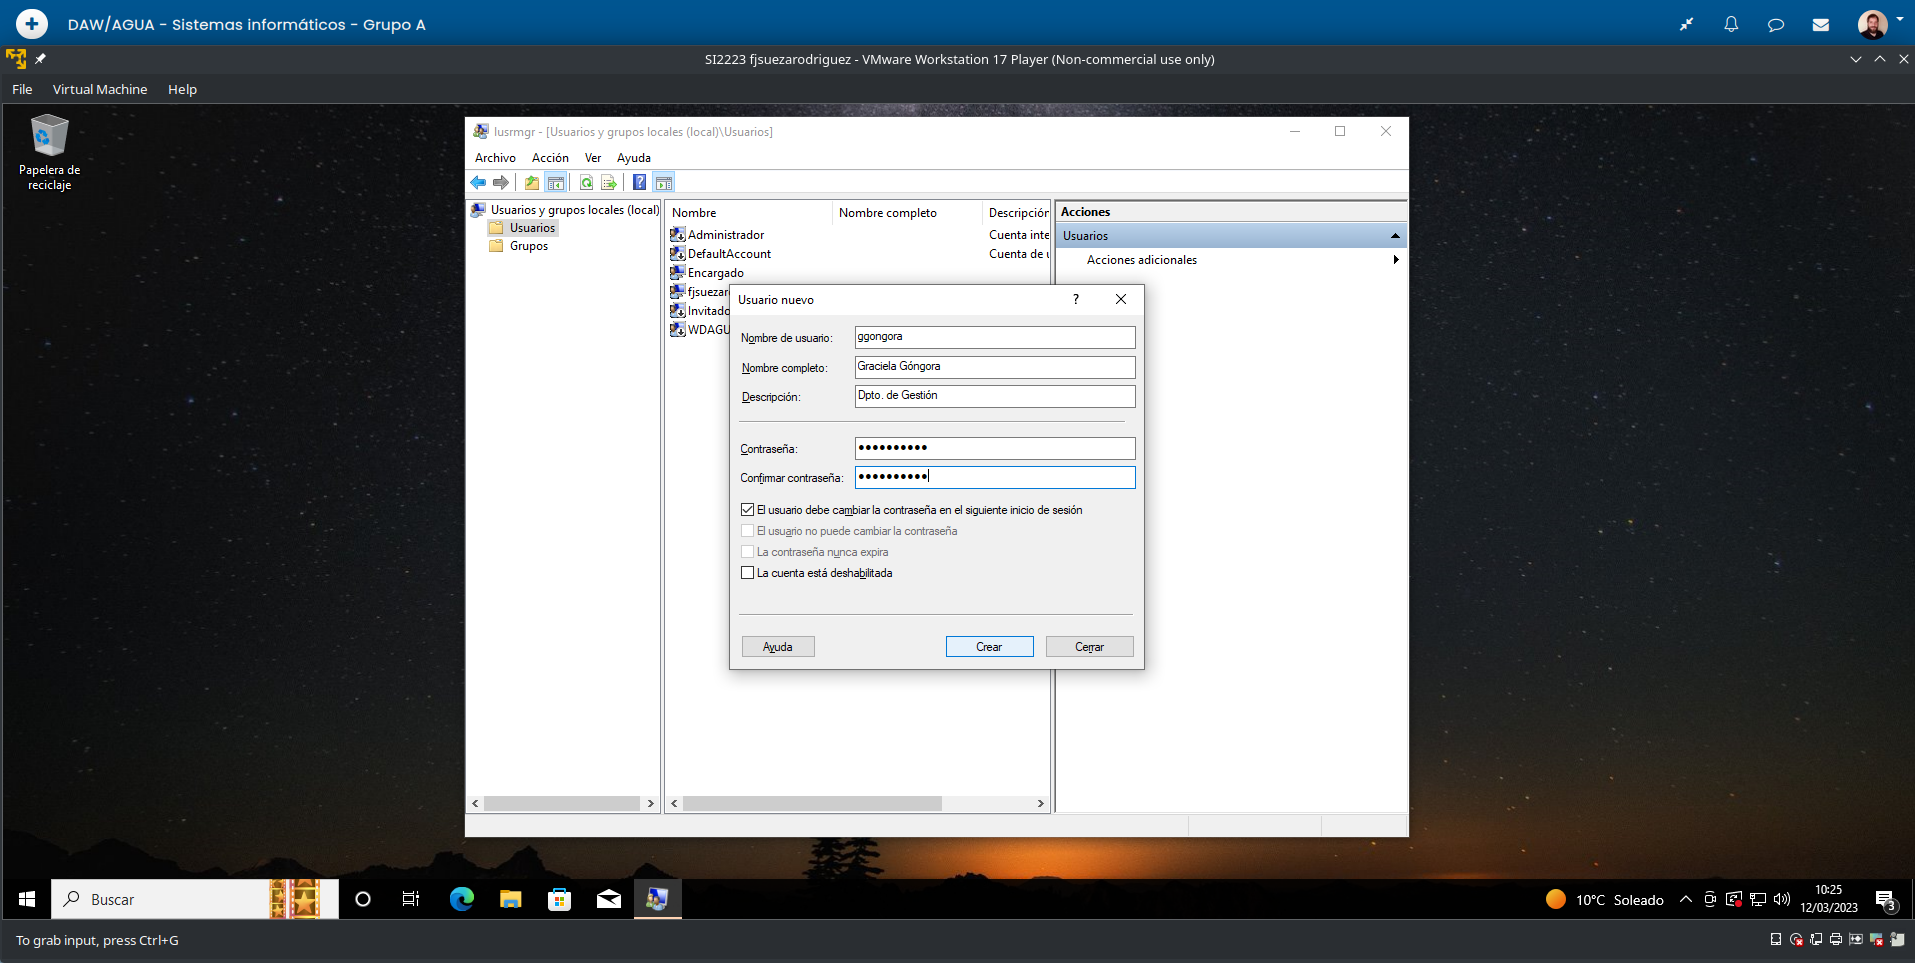
\includegraphics[scale=0.22]{usuarios-datos.png}
        \caption{Introducción de datos de usuario}
    \end{figure}

    Tras haber creado los 4 usuarios que se piden, las cuentas de usuario que tenemos en el sistema las podemos ver en la ventana principal de \textbf{lusrmgr}, como vemos en la siguiente captura.

    \begin{figure}[H]
        \centering
        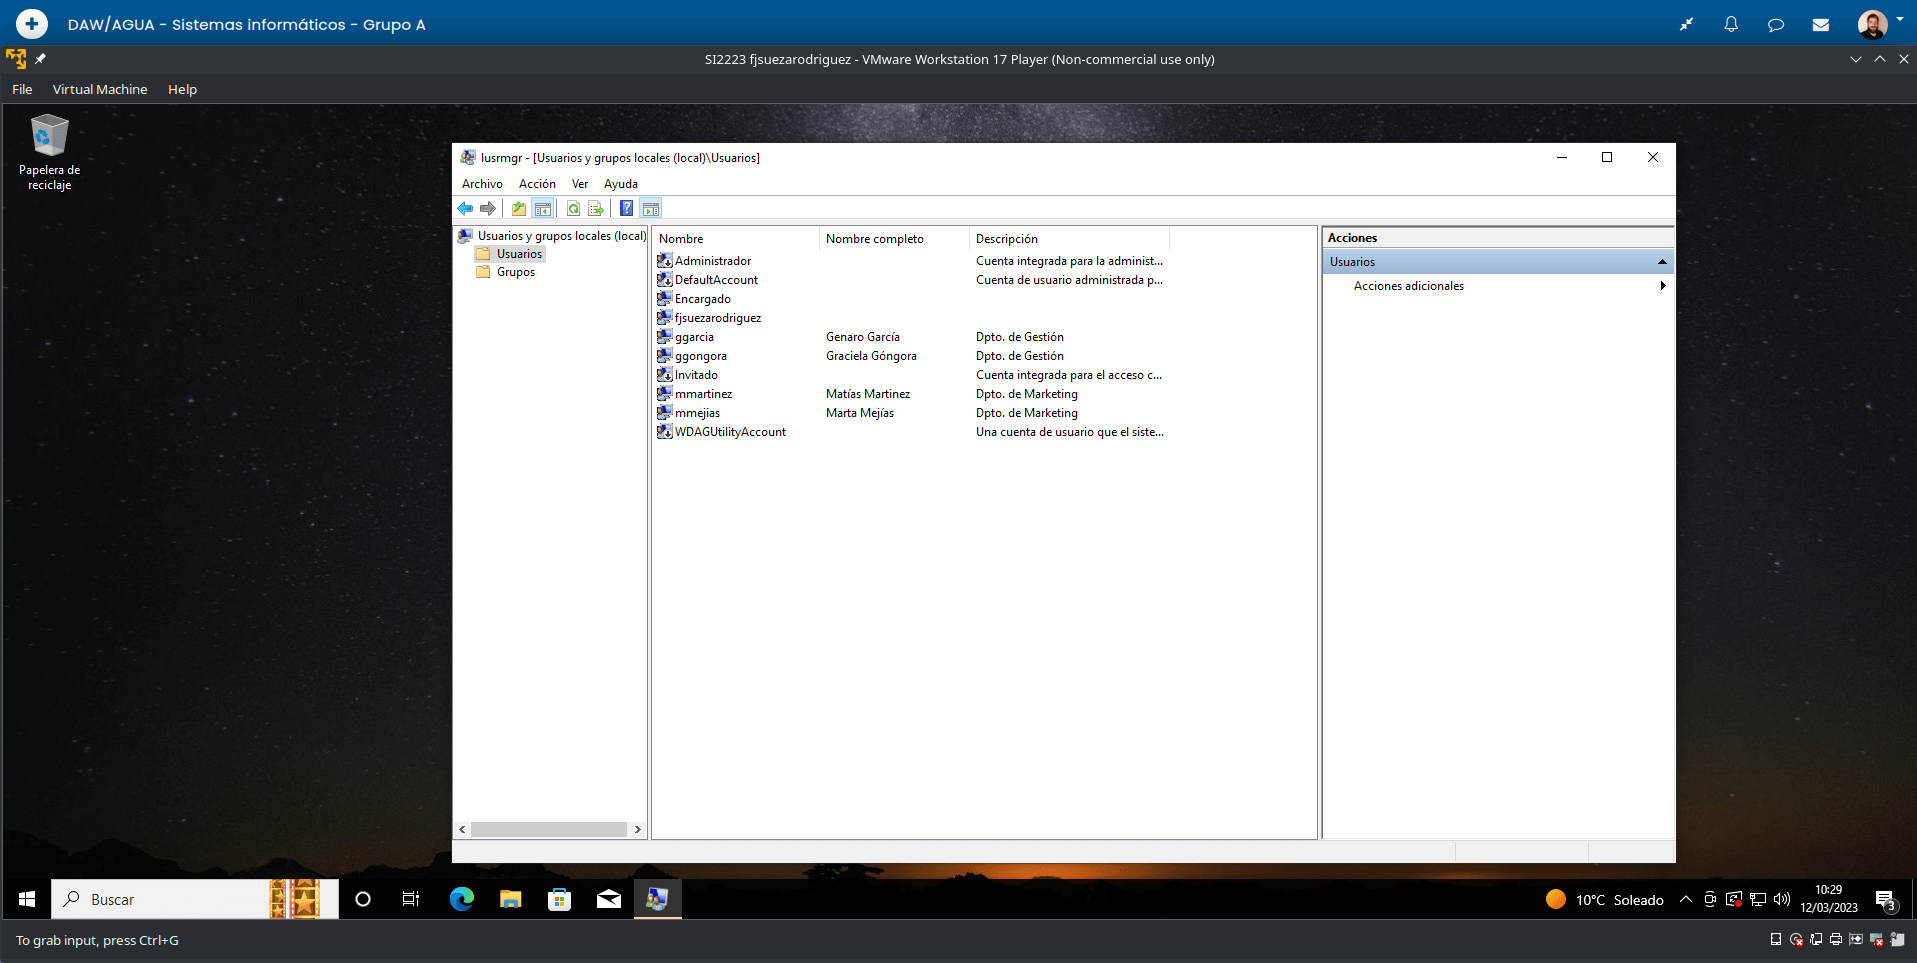
\includegraphics[scale=0.18]{usuarios-creados.png}
        \caption{Usuario creados con lusrmgr}
    \end{figure}

    \item En segundo lugar vamos a \textbf{crear los grupos} que se nos piden y añadir a ellos los usuarios pertinentes. Para esa tarea vamos a usar también la aplicación \textbf{lusrmgr}, tal y como hemos hecho en el punto anterior. La forma de acceso a la aplicación es la misma que en punto anterior, la única diferencia es que hemos pulsado en la opción \textbf{Grupos} del menú de la izquierda una vez abierta esta.

    \begin{figure}[H]
        \centering
        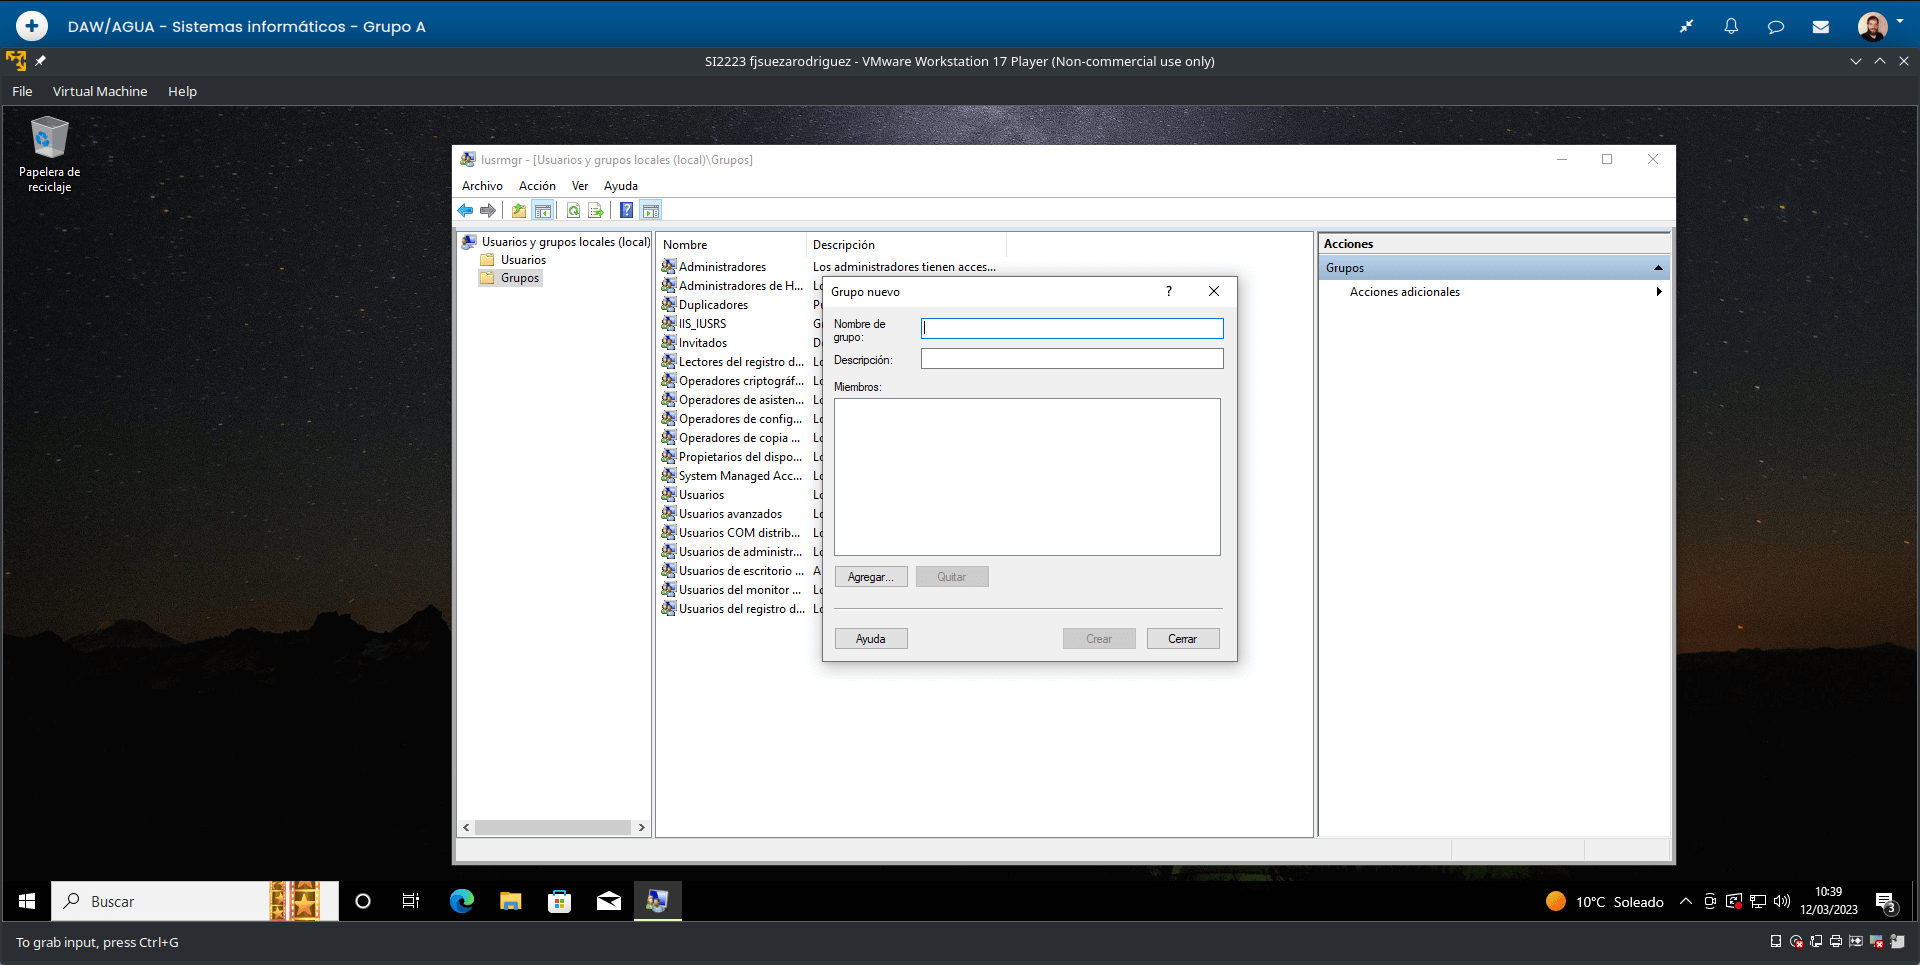
\includegraphics[scale=0.18]{grupos-creaci.png}
        \caption{Ventana de creación de un nuevo grupo}
    \end{figure}

    Una vez que estamos en esta ventana, podemos introducir los diferentes datos que se nos piden, como es el nombre del grupo y su descripción.

    \begin{figure}[H]
        \centering
        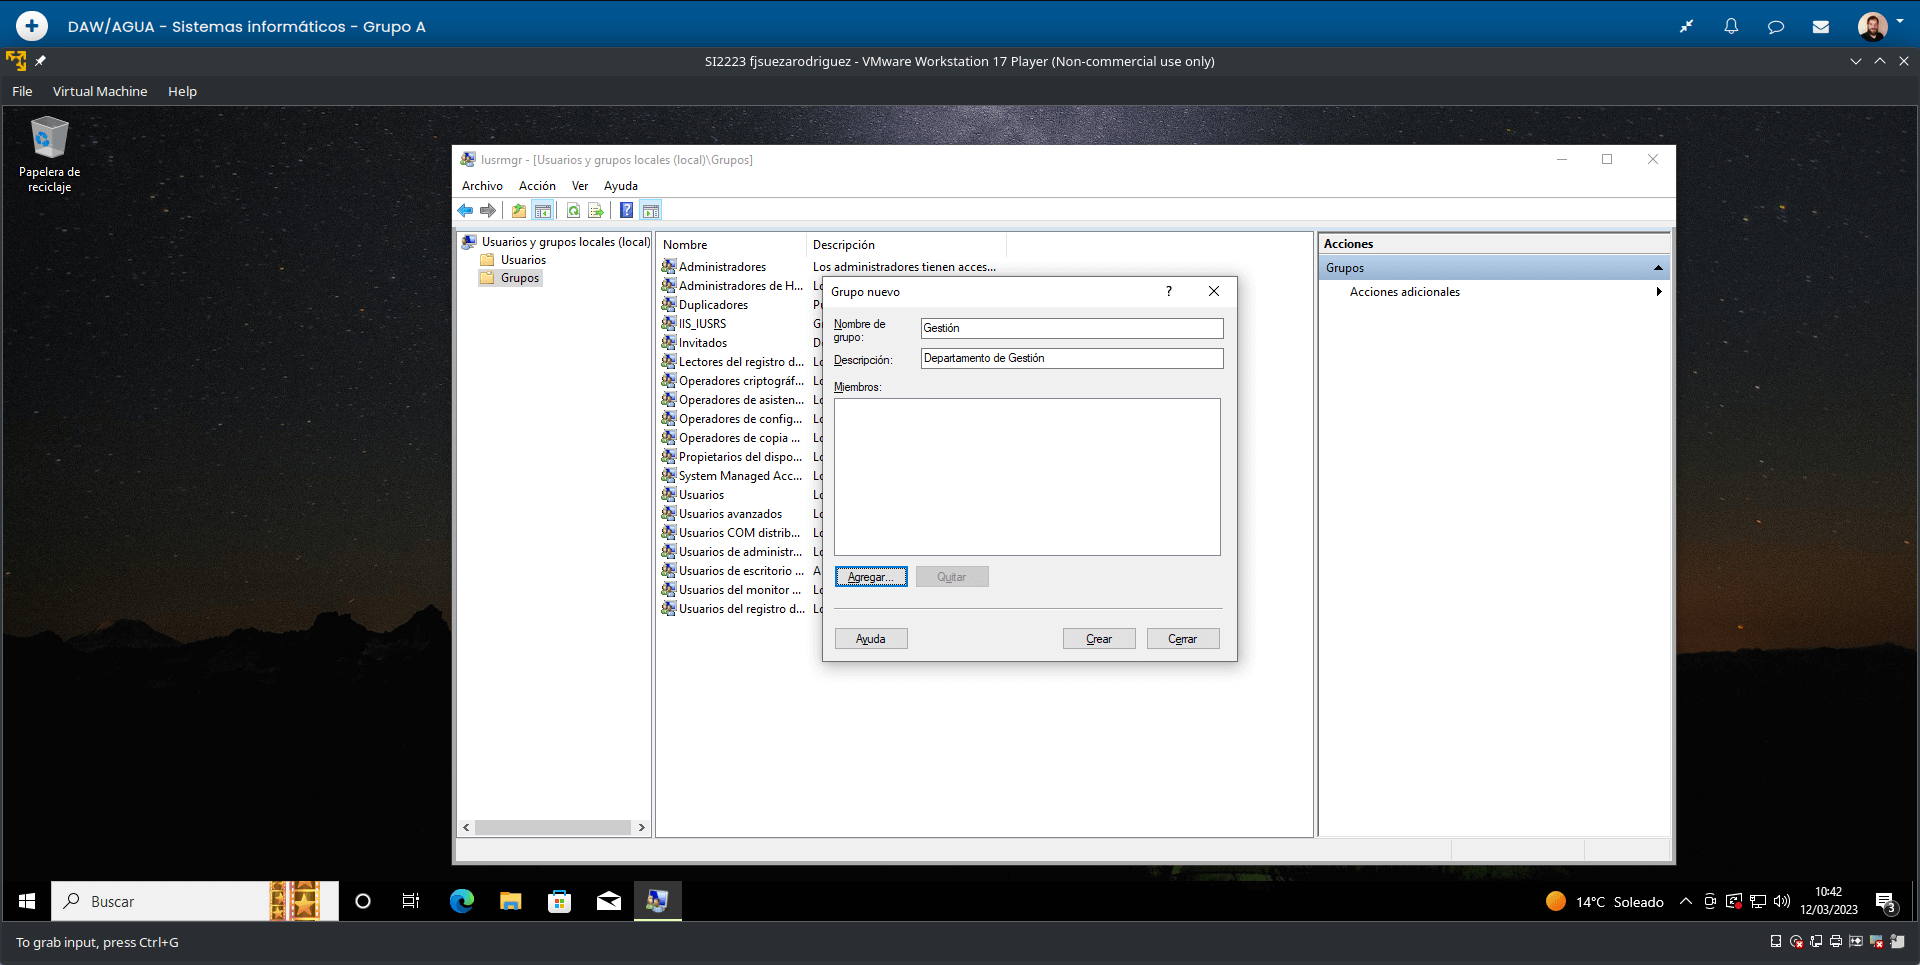
\includegraphics[scale=0.18]{grupos-datos.png}
        \caption{Introducción de datos del nuevo grupo}
    \end{figure}

    En esta misma ventana, podemos agregar los usuarios pertenecientes a dicho grupos, pulsando en el botón \textbf{Agregar} e introduciendo el nombre del usuario en cuestión.

    \begin{figure}[H]
        \centering
        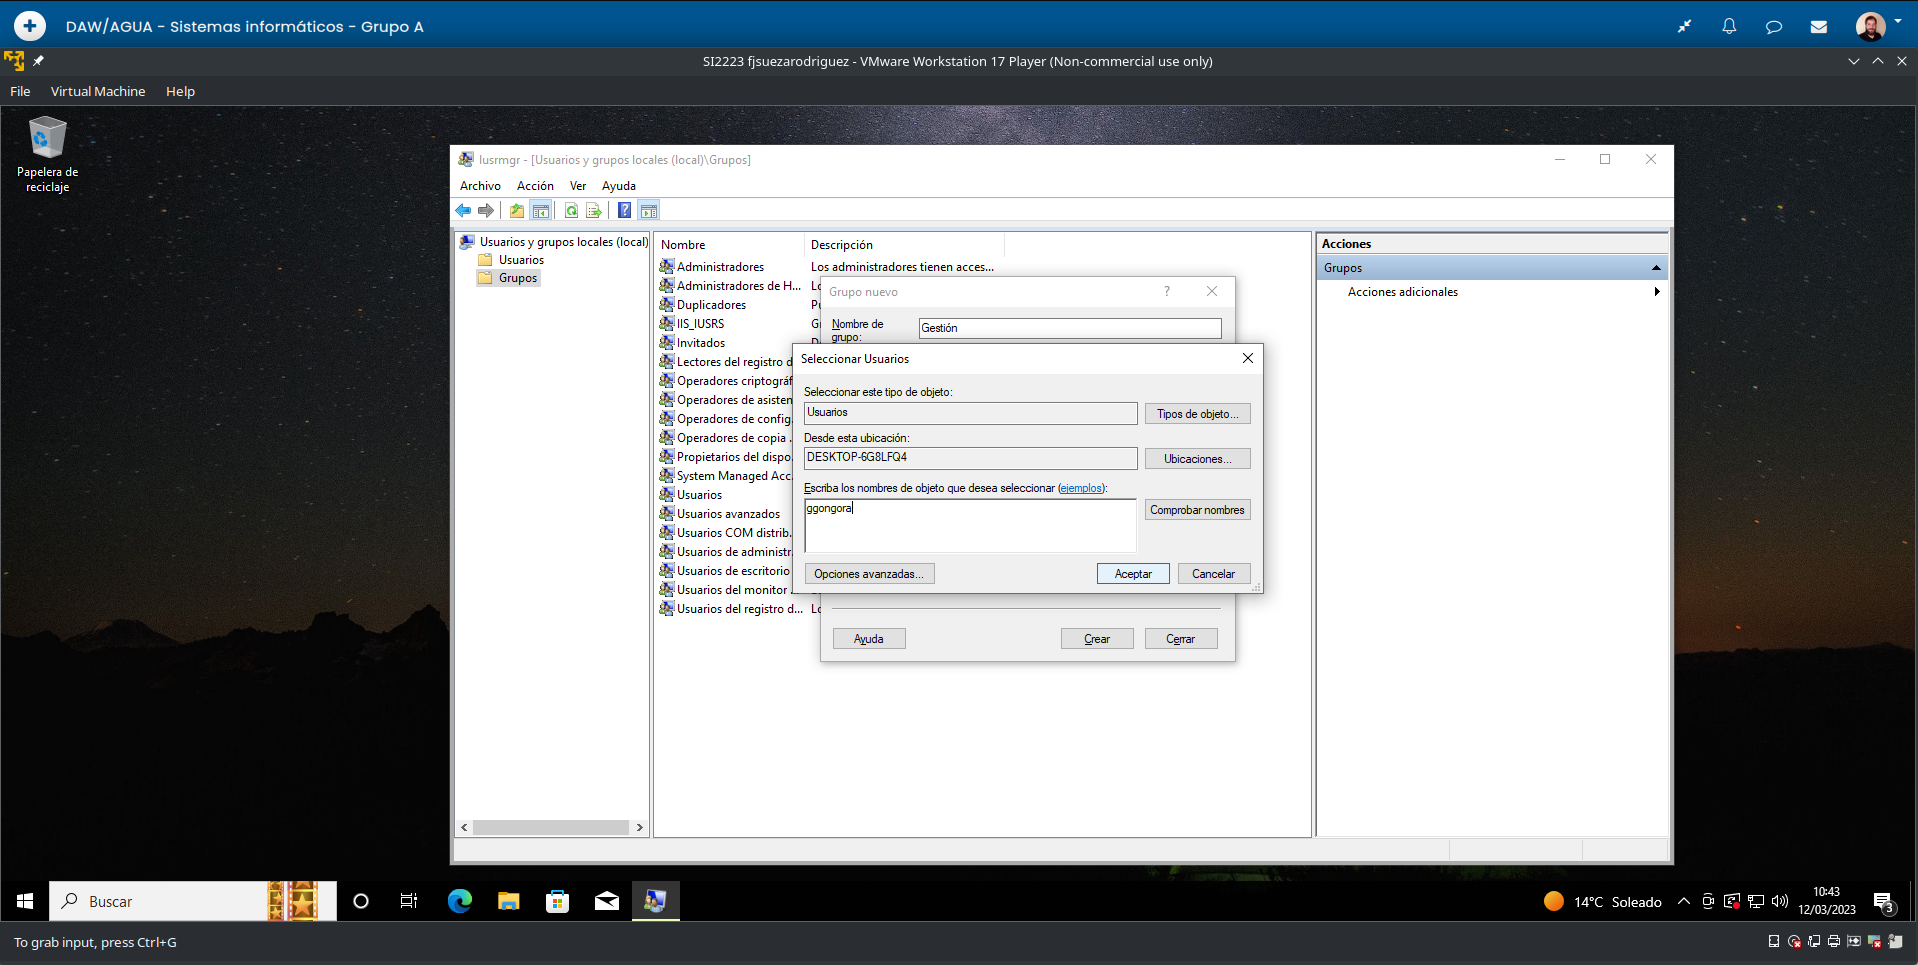
\includegraphics[scale=0.20]{grupos-usuarios.png}
        \caption{Agregación de un usuario al grupo}
    \end{figure}

    Una vez creados los dos grupos y agregados los usuarios que pertenecen a cada uno, estos han quedado como se puede ver en las siguientes dos capturas.

    \begin{figure}[H]
        \centering
        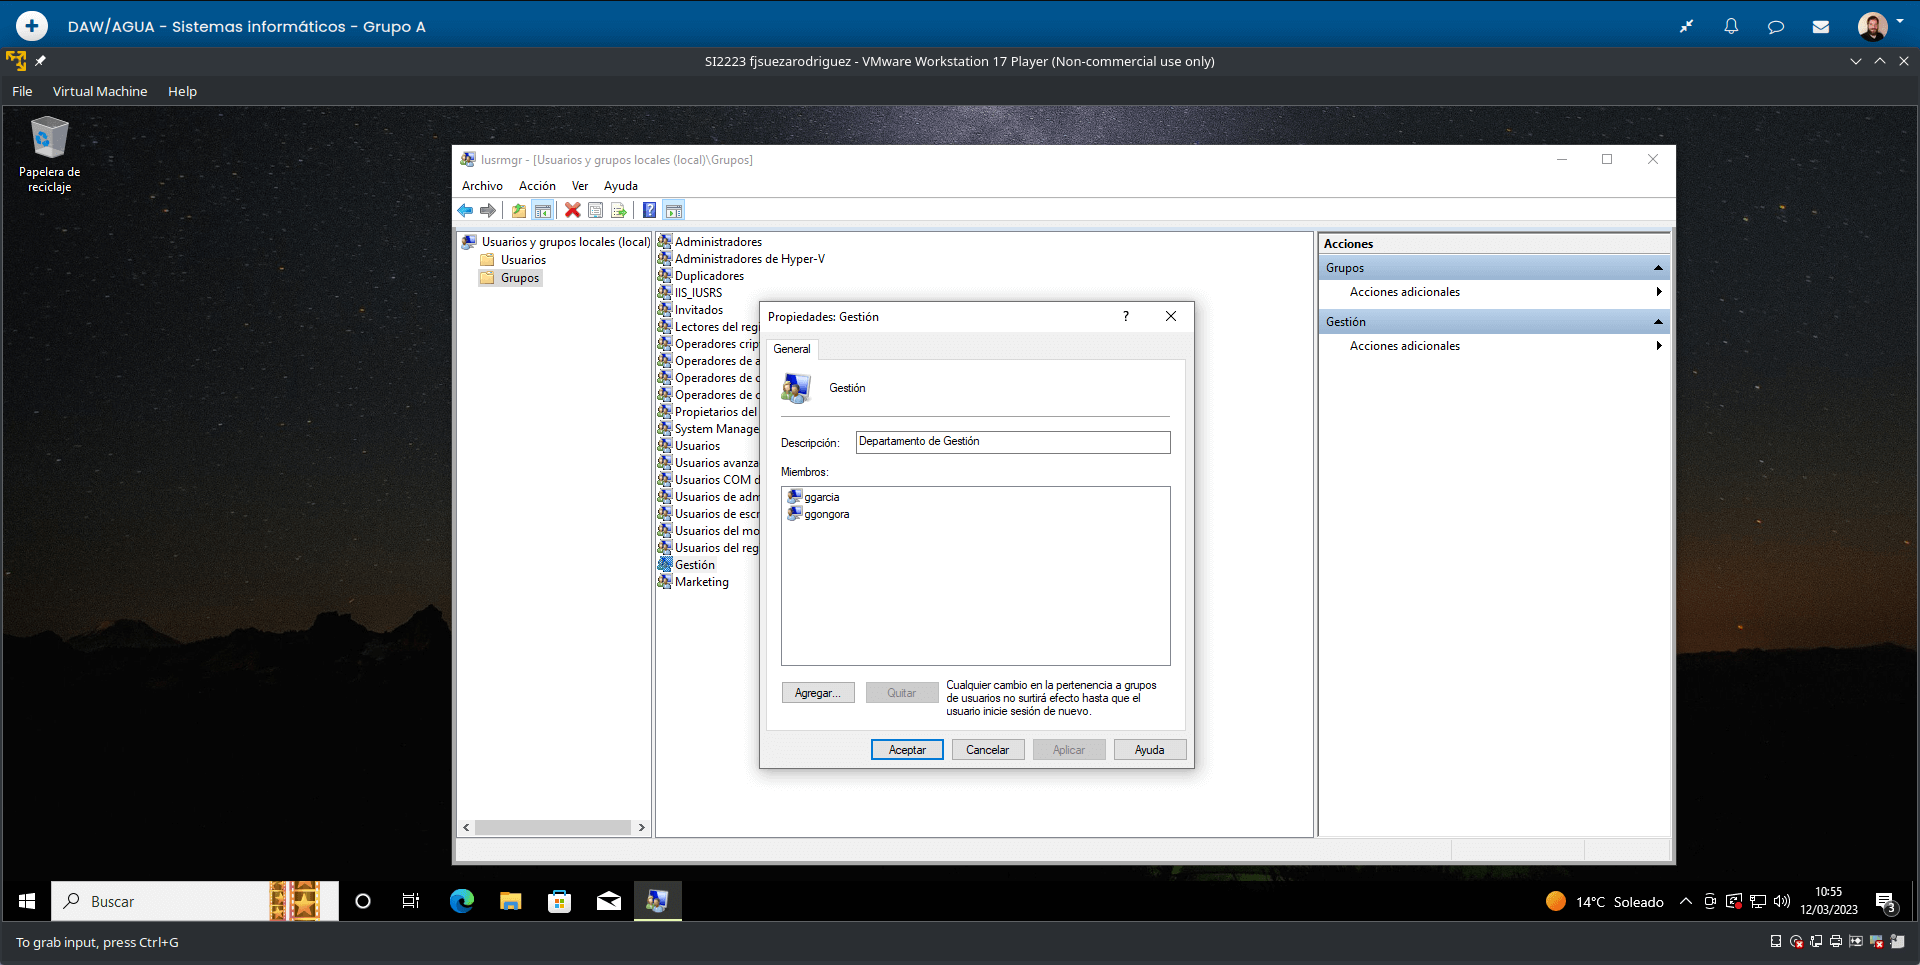
\includegraphics[scale=0.20]{grupos-gestion.png}
        \caption{Grupo Gestión creado}
    \end{figure}

    \begin{figure}[H]
        \centering
        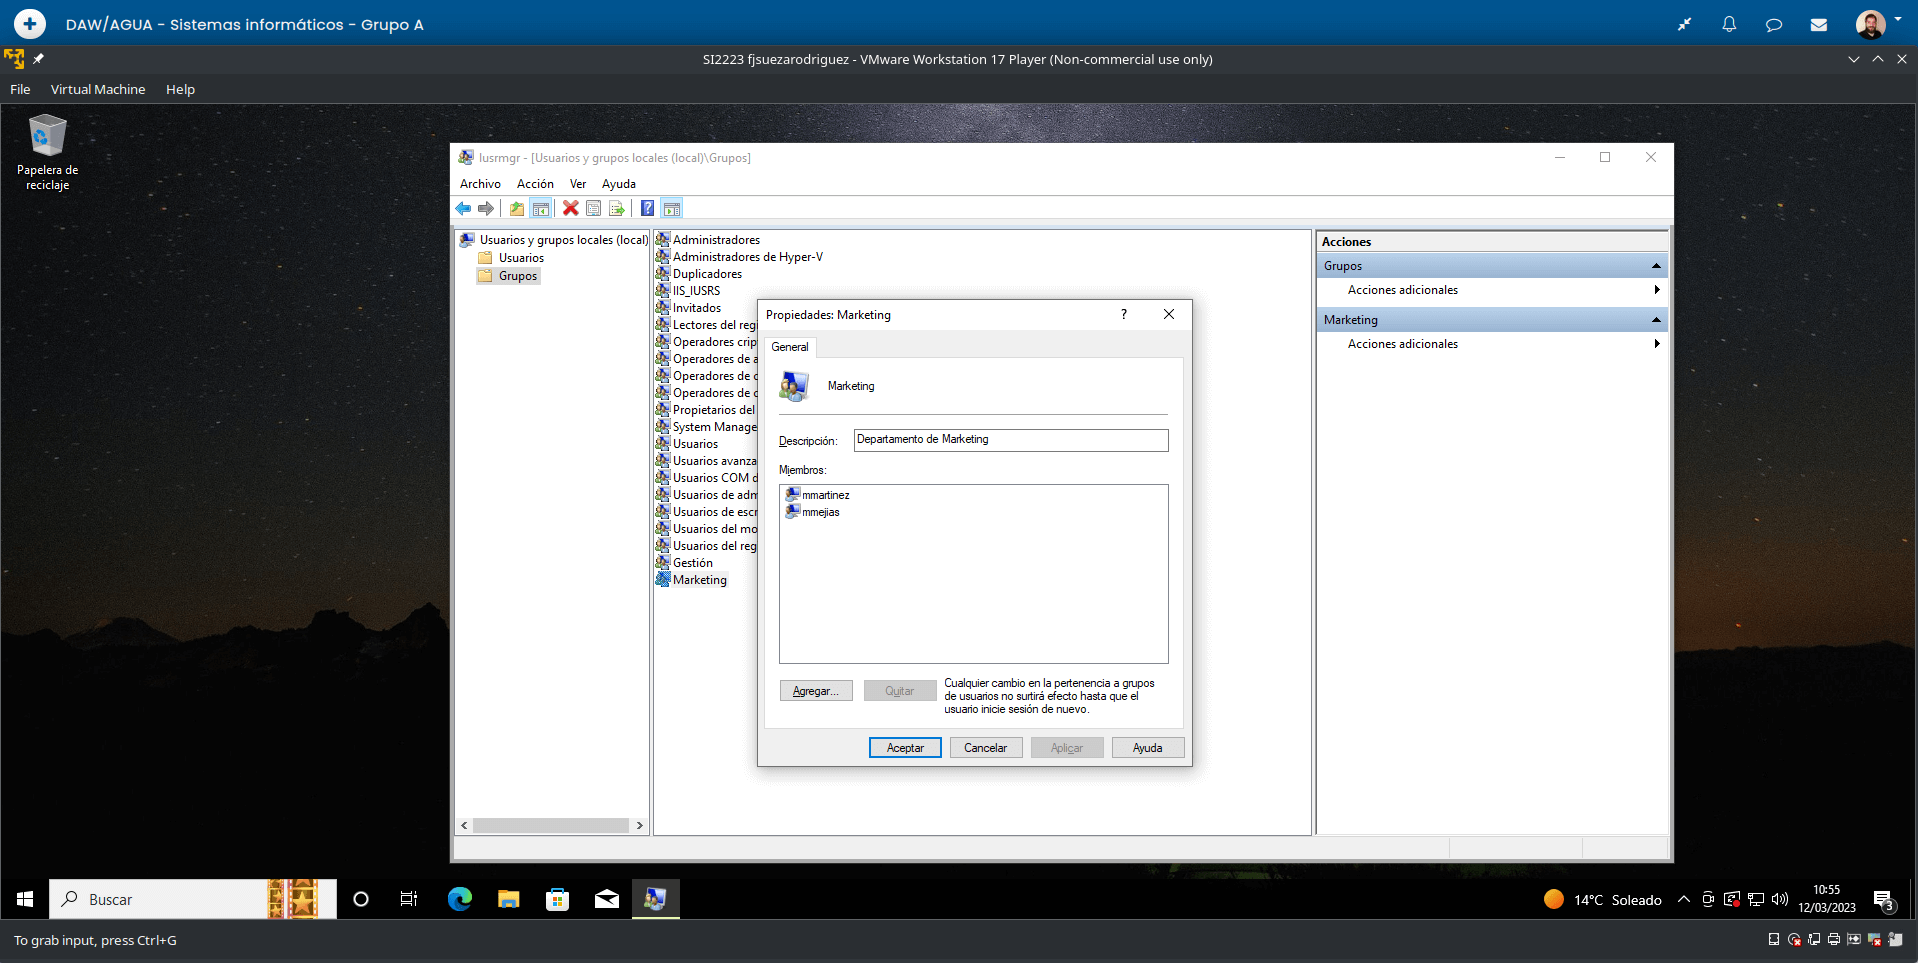
\includegraphics[scale=0.20]{grupos-marketing.png}
        \caption{Grupo Marketing creado}
    \end{figure}
\end{enumerate}

\subsection{Actividad 3: Permisos de Archivos y Carpetas}

\subsubsection{Enunciado}
Configura los permisos de las carpetas creadas en la primera actividad, para que los usuarios creados en la segunda actividad, tengan permisos de lectura y escritura sobre la carpeta de su departamento. El resto de usuarios, aunque se cree posteriormente en el sistema, no tendrá ningún acceso si no pertenece a ese departamento. Los permisos se asignarán a los grupos que creaste en la actividad 2.b, no a los usuarios de manera individual.

A continuación, para comprobar que los permisos aplicados son correctos, inicia sesión con un usuario de un departamento, intenta acceder a la carpeta de su departamento y a la del otro departamento, e indica qué ocurre en cada caso. Realiza también la comprobación de acceder con el usuario creado en la instalación de Windows 10 a las carpetas de los departamentos.

\textbf{Capturas}:

\begin{itemize}
    \item Ventana donde se asignan los permisos de la carpeta ``Gestión'' (indica textualmente cómo se accede a dicha ventana).
    \item Proceso de asignación de permisos a la carpeta ``Gestión''. Deben mostrarse los nombres de los grupos implicados sus respectivos permisos.
    \item Resumen de la asignación de permisos a la carpeta ``Marketing''. Deben mostrarse los nombres de los grupos implicados y sus respectivos permisos.
    \item Acceso de un usuario de un departamento a la carpeta de su departamento y a la del otro departamento.
    \item Acceso del usuario creado en la instalación de Windows 10 a las carpetas de los departamentos.
\end{itemize}

\subsubsection{Solución}

En esta actividad vamos a cambiar los permisos de las carpetas creadas en la Actividad 1 para que solo los usuarios pertenecientes a dichos departamentos puedan acceder a ellos y modificarlos. Para ellos hemos realizado los siguientes pasos.

\begin{enumerate}
    \item Primero hemos modificado los permisos del directorio \textbf{Gestión}. Para ello, nos hemos situado en su directorio padre, \textbf{AguadulSoft}, y hemos hecho click con el \textbf{botón derecho} sobre el directorio y pulsado en la opción \textbf{Propiedades} del menú que se nos despliega. A continuación, hemos pulsado en la pestaña \textbf{Seguridad}.

    \begin{figure}[H]
        \centering
        \includegraphics[scale=0.19]{permisos-gestión.png}
        \caption{Ventana con permisos de la carpeta Gestión}
    \end{figure}

    Hay que tener en cuenta, que ahora mismo no podemos modificar estos permisos. Para ello deberemos modificar la opción de \textbf{herencia} en \textbf{Opciones avanzadas}, pulsando en el botón \textbf{Deshabilitar Herencia}. En la ventana que se nos muestra, deberemos elegir la opción para \textbf{Hacer los permisos heredados explícitos}, lo que nos permitirá modificar los permisos del directorio sin eliminar los que ya tiene, ya que hay ciertos grupos como \textbf{SYSTEM} o \textbf{Administradores} que nos interesa mantener dentro de los grupos que pueden modificar el directorio.

    Una vez hecho esto, hemos vuelta a la ventana anterior y pulsado en la opción \textbf{Editar} para eliminar y añadir los grupos oportunos, como podemos ver en la siguiente captura.

    \begin{figure}[H]
        \centering
        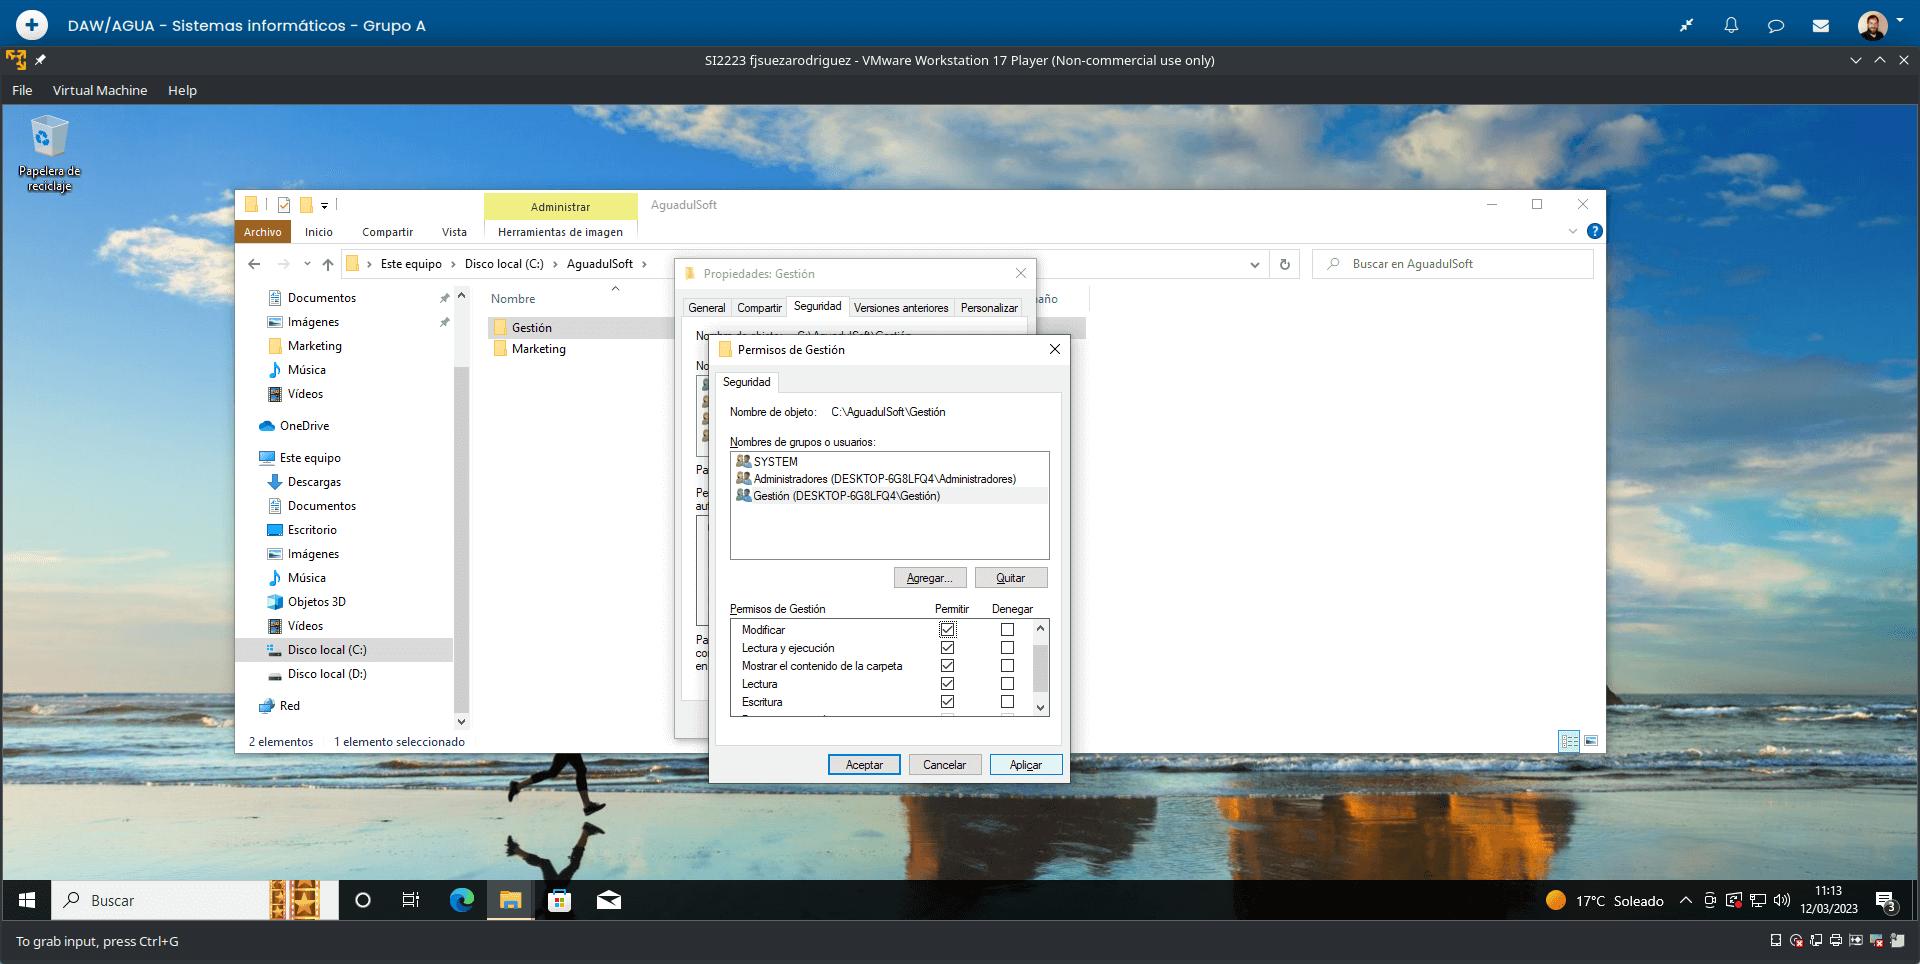
\includegraphics[scale=0.20]{permisos-gestion-nuevos.png}
        \caption{Modificación de los permisos de la carpeta Gestión}
    \end{figure}

    \item A continuación, hemos realizado el mismos procedimiento en la carpeta \textbf{Marketing}, quedando después de la modificación como vemos en la siguiente figura.

    \begin{figure}[H]
        \centering
        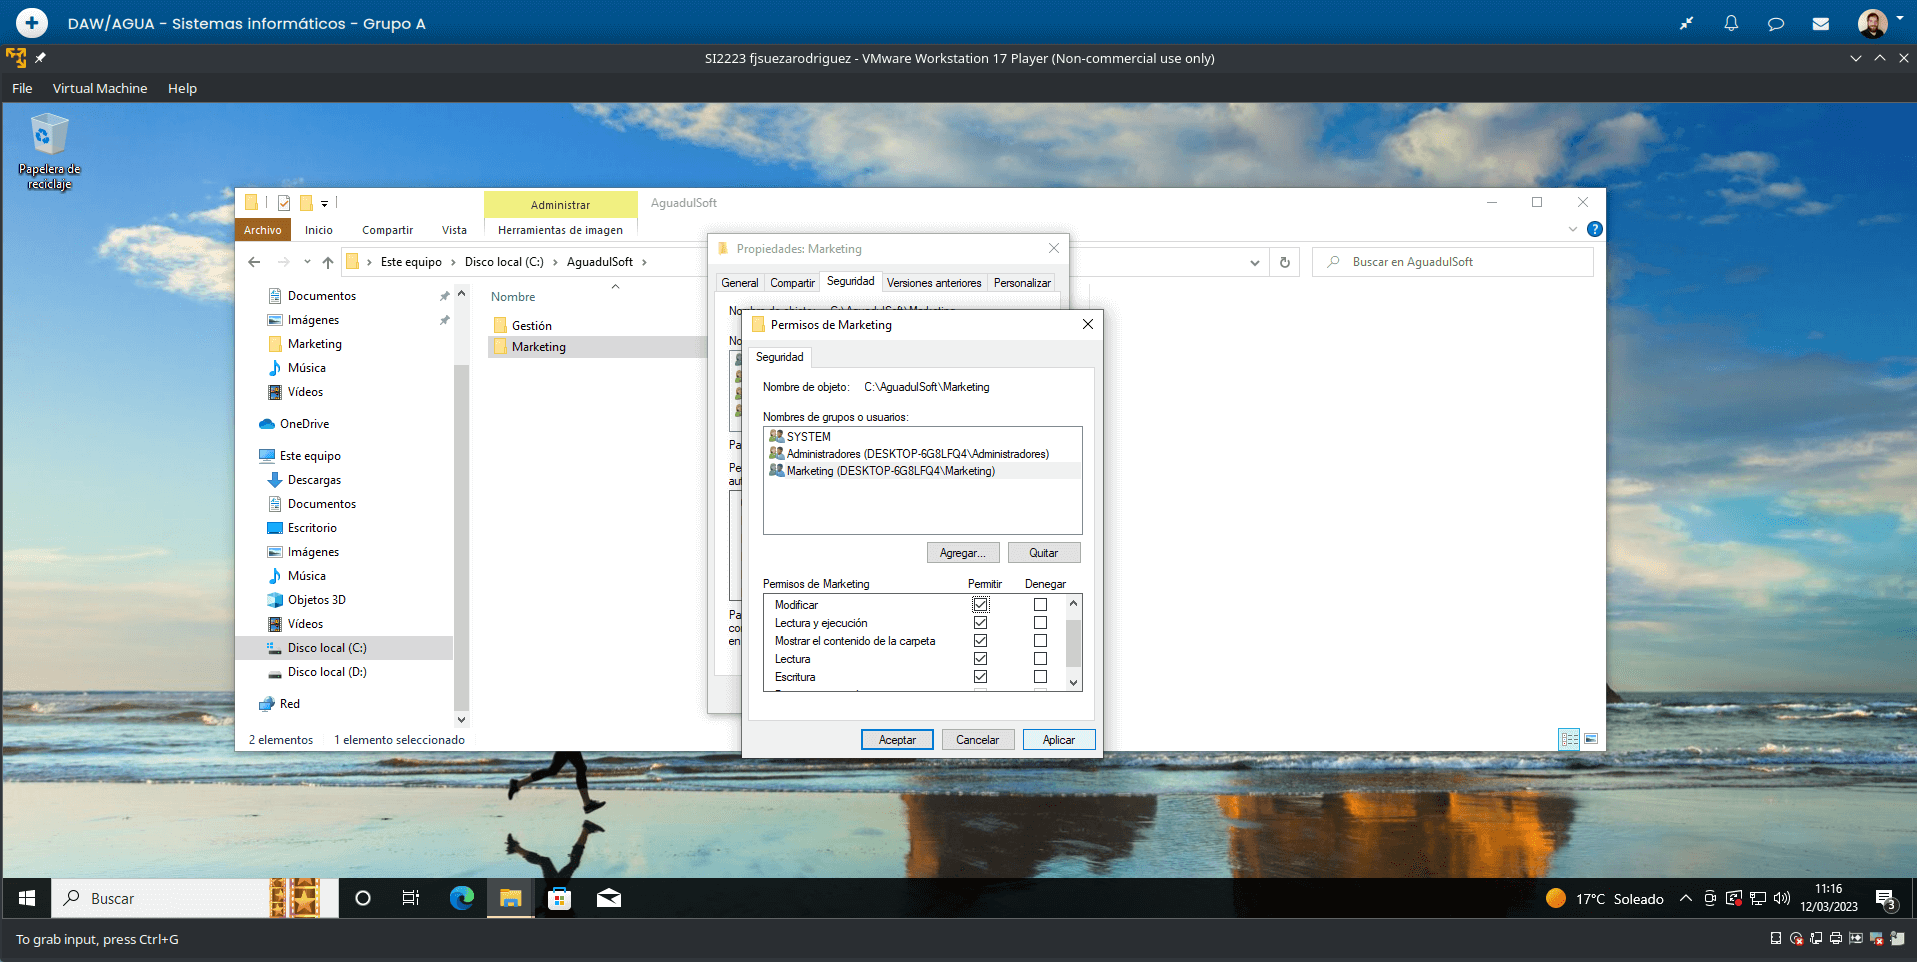
\includegraphics[scale=0.20]{permisos-marketing.png}
        \caption{Modificación de los permisos de la carpeta Marketing}
    \end{figure}

    \item Por último, para \textbf{comprobar que los cambios} se han \textbf{realizado correctamente}, hemos intentado acceder a dichas carpetas con \textbf{usuarios que deberían tener permiso}s y con \textbf{usuarios que no deberían} tenerlos. Hay que tener en cuenta que si el usuario que usamos tiene permisos de administrador se le va a poder habilitar en el directorio concreto, ya que los administrador han conservado sus permisos en dichos directorios.

   Primero hemos intentado acceder a la \textbf{carpeta Gestión} con un \textbf{usuario} perteneciente al \textbf{grupo Gestión}, intentando, posteriormente, acceder con este usuario a la \textbf{carpeta Marketing}. Hemos elegido el usuario \textbf{ggongora}.

   \begin{figure}[H]
       \centering
       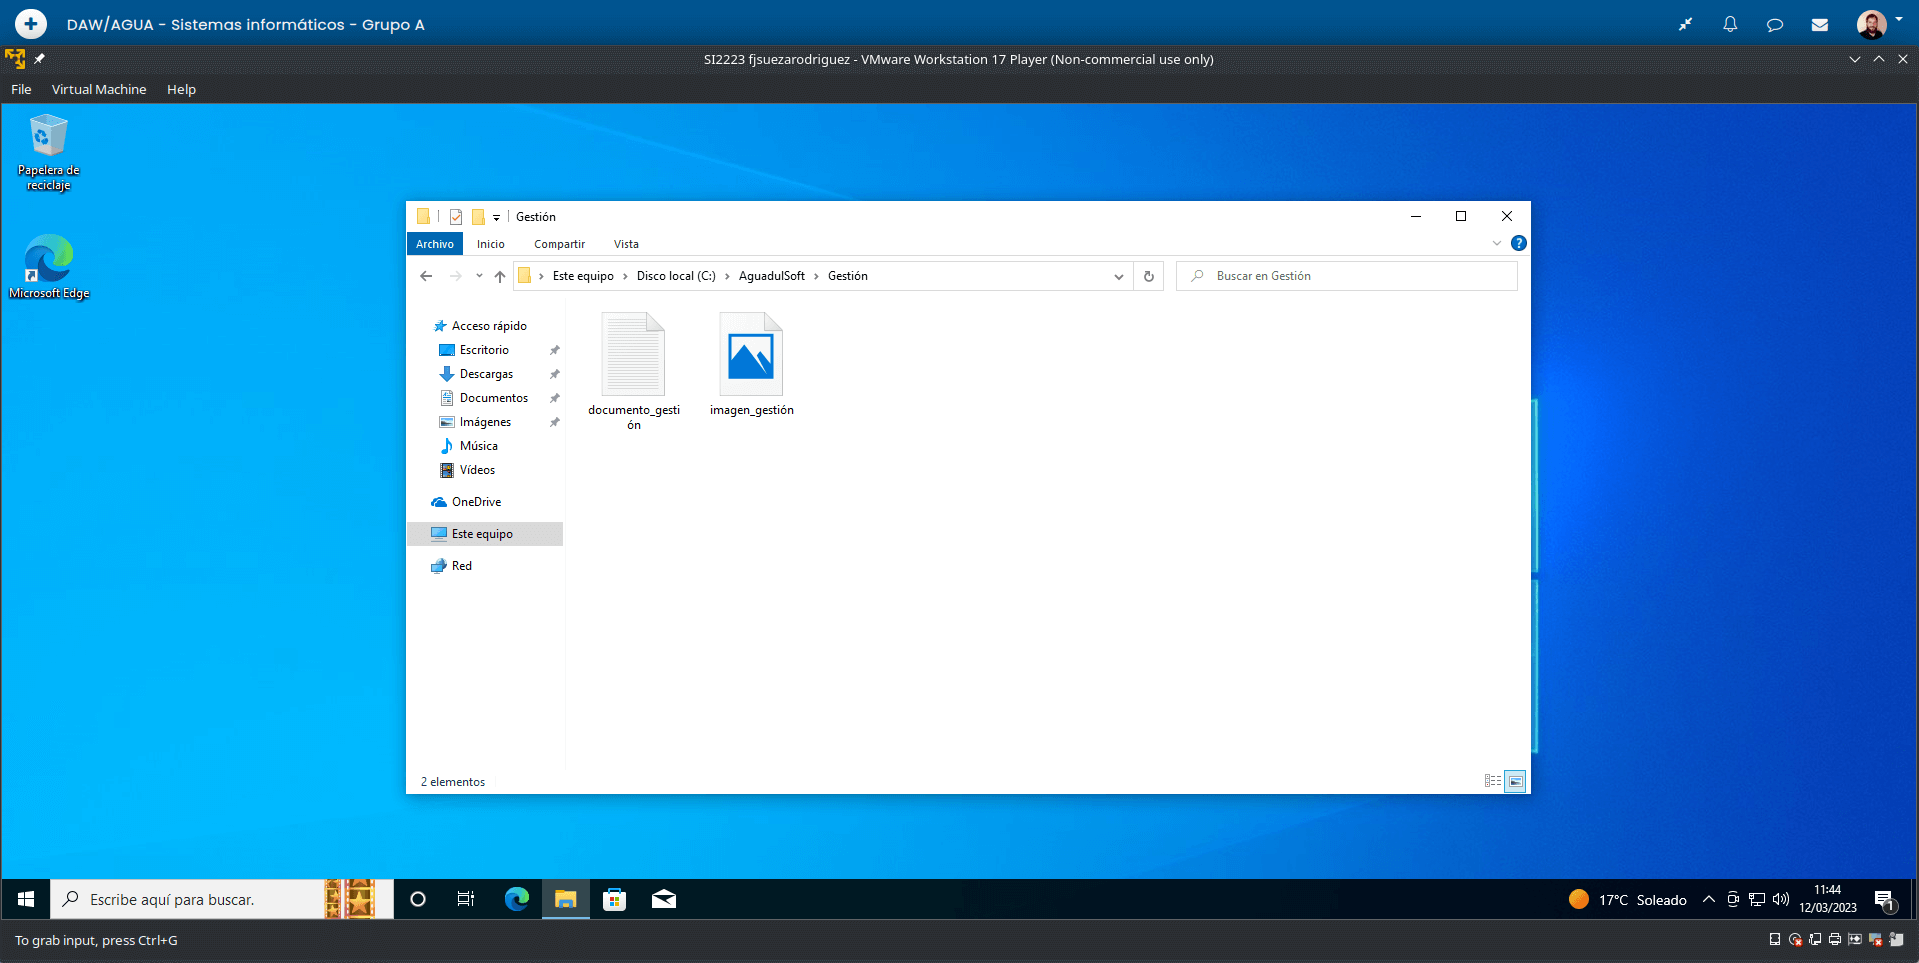
\includegraphics[scale=0.20]{permisos-test-1.png}
       \caption{Acceso a la carpeta Gestión con la usuaria ggongora}
   \end{figure}

    En este caso, \textbf{no hemos tenido ningún problema} de acceder a la carpeta Gestión. Ahora vamos a intentar acceder a la carpeta \textbf{Marketing}.

    \begin{figure}[H]
        \centering
        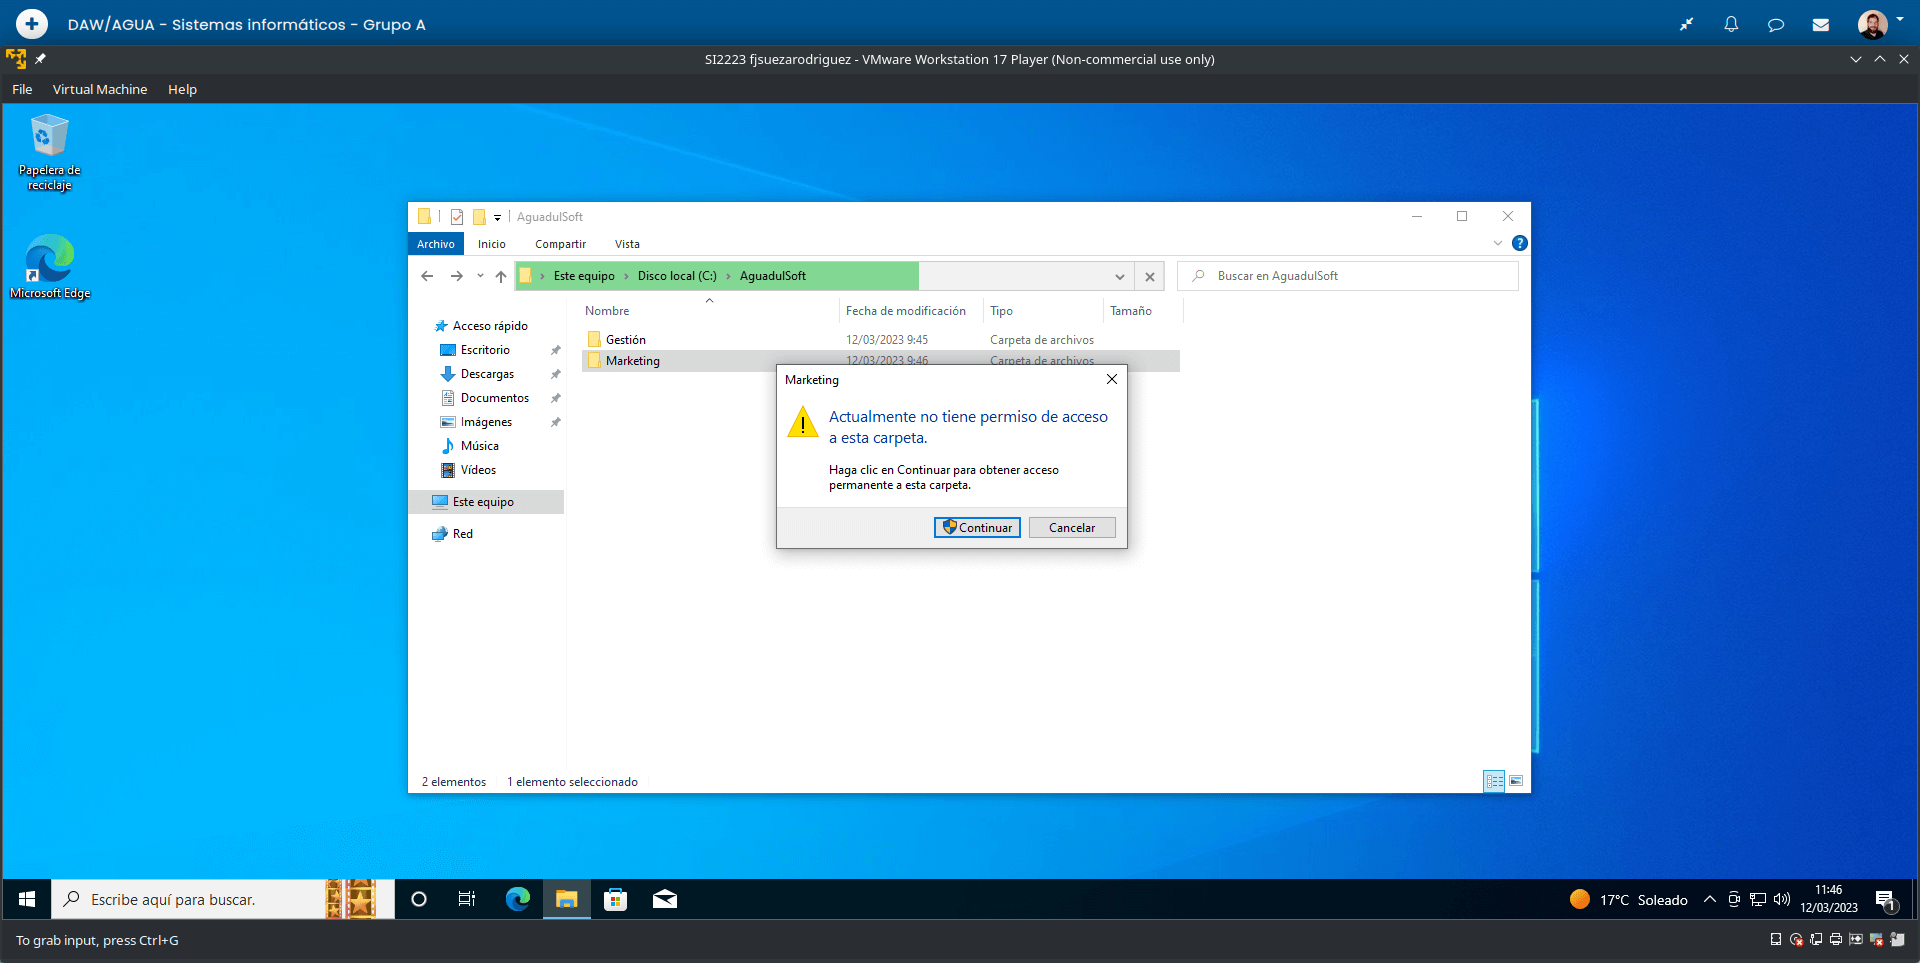
\includegraphics[scale=0.20]{permisos-test-2.png}
        \caption{Acceso a la carpeta Marketing con la usuaria ggongora}
    \end{figure}

    Como vemos, se nos muestra una ventana informándonos de que no tenemos permisos. Como los administradores si los tienen, nos da la opción de agregarnos para tener permisos en esa carpeta, pero como \textit{no sabemos la contraseña de administrador}, no podemos hacerlo. Por último, probamos a entrar en las carpetas con el \textbf{usuario creado} durante \textbf{la instalación} de Windows 10.

   \begin{figure}[H]
        \centering
        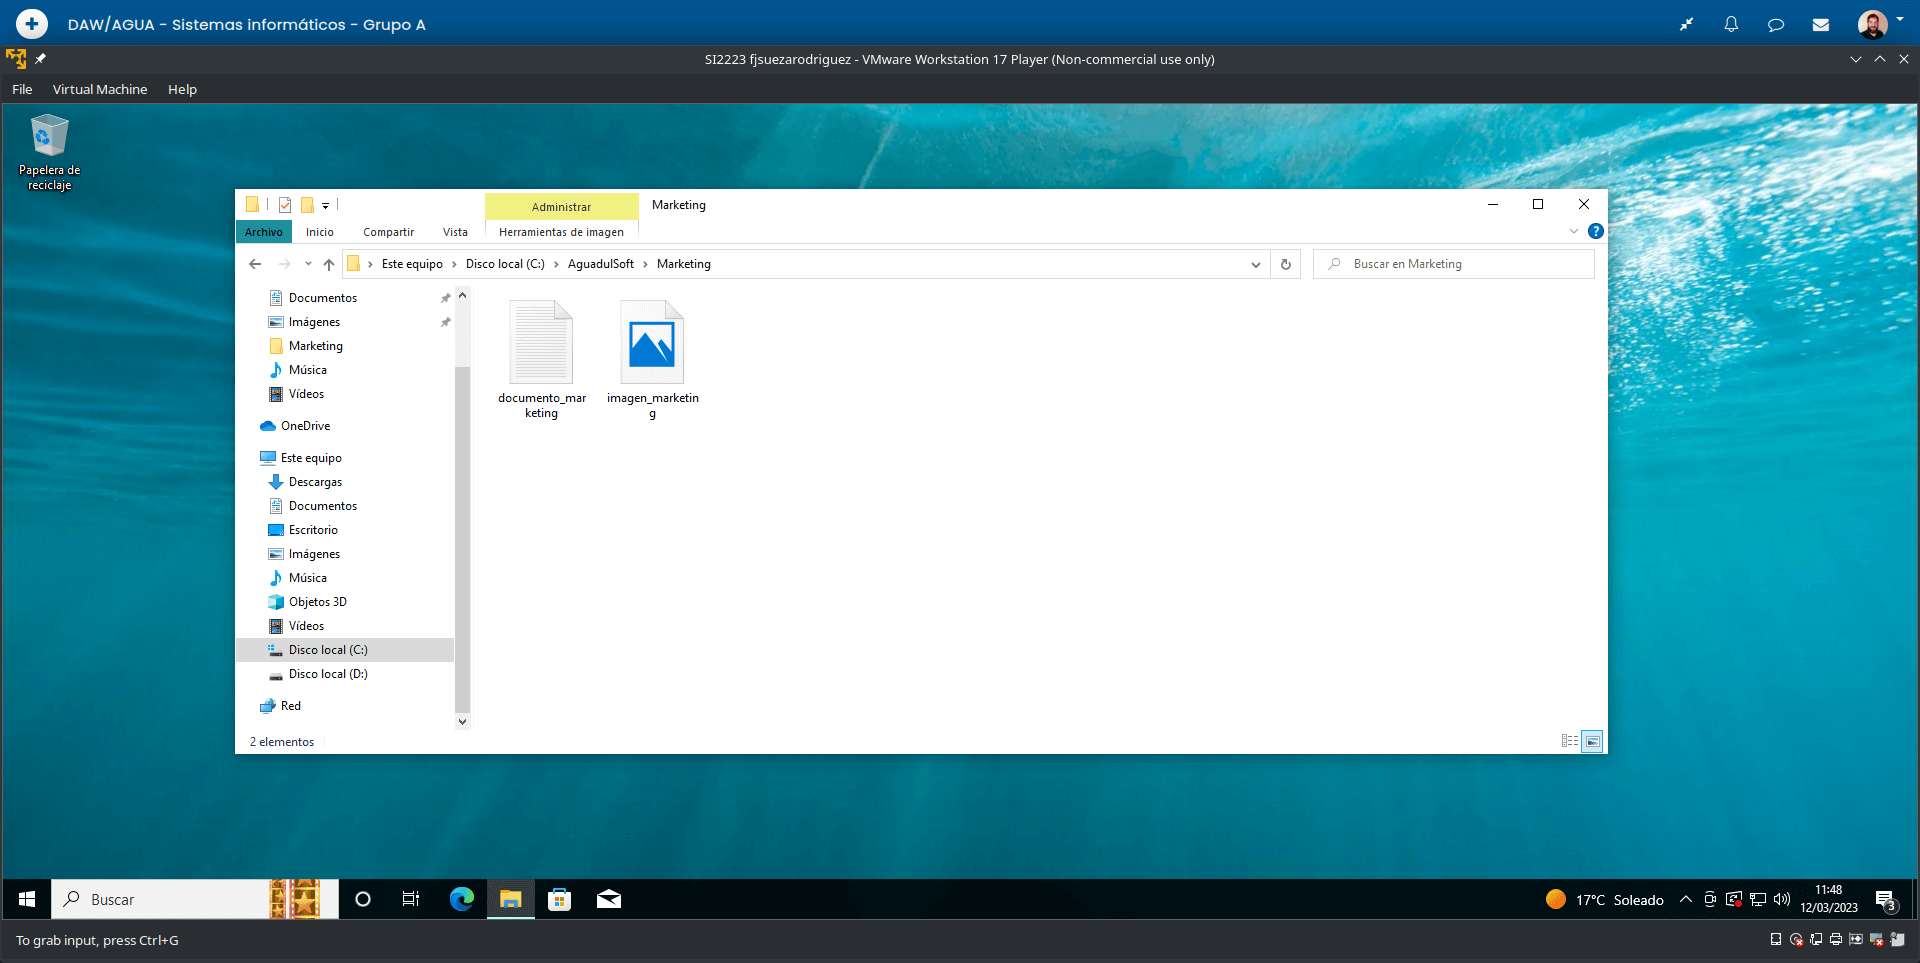
\includegraphics[scale=0.20]{permisos-test-3.png}
        \caption{Acceso a las carpetas con el usuario creado en la instalación}
    \end{figure}

    Como este usuario \textbf{sí tiene permisos de administrador}, no tenemos problemas en acceder a ninguna de las carpetas.
\end{enumerate}



% Bibliography

\newpage
\bibliography{citas}
\bibliographystyle{unsrt}

\end{document}